\documentclass[a4paper,10pt]{jsarticle}

% レイアウト
\setlength{\textwidth}{\fullwidth}
\setlength{\textheight}{39\baselineskip}
\addtolength{\textheight}{\topskip}
\setlength{\voffset}{-0.5in}
\setlength{\headsep}{0.3in}
\pagestyle{myheadings}

% パッケージ
\usepackage[dvipdfmx]{graphicx}
\usepackage{amsmath,amssymb,epsfig}
\usepackage{bm}
\usepackage{ascmac}
\usepackage{pifont}
\usepackage{multirow}
\usepackage{enumerate}
\usepackage{cases}
\usepackage{type1cm}
\usepackage{cancel}
\usepackage{url}
\usepackage{listings,jlisting}
% 大きな中括弧
\usepackage{cases}


% カウンタの設定
\setcounter{section}{0}
\setcounter{subsection}{0}
\setcounter{subsubsection}{0}
\setcounter{equation}{0}

% キャプションの図をFigに変更
\renewcommand{\figurename}{Fig.}
\renewcommand{\tablename}{Tab.}

% 式番号を式(章番号.番号)に
\makeatletter
\renewcommand{\theequation}{\arabic{section}.\arabic{equation}}
\@addtoreset{equation}{section}
\makeatother

% 表紙
\title{知能システム学特論レポート}
\author{
(DL2班)Caffe on Ubuntu\\
}
\date{2015年\ 6月\ 22日}

% ドキュメントの開始
\begin{document}
\maketitle
\section{報告者}
\begin{list}{}{}
 \item 15344203\hspace{0.5cm} 有田 裕太
 \item 15344206\hspace{0.5cm} 緒形 裕太
 \item 15344209\hspace{0.5cm} 株丹 亮
 \item 12104125\hspace{0.5cm} 宮本 和
\end{list}

\section{進行状況}
サンプルを実行することができた.

\subsection{サンプルの実行}

分類する画像を指定
\begin{lstlisting}[basicstyle=\ttfamily\footnotesize, frame=single]
python classify.py --raw_scale 255 ../examples/images/cat.jpg ./result.npy
\end{lstlisting}

サンプル画像をFig.\ref{sample1}〜\ref{sample3}に示す.

\begin{figure}[b]
 \centering	
    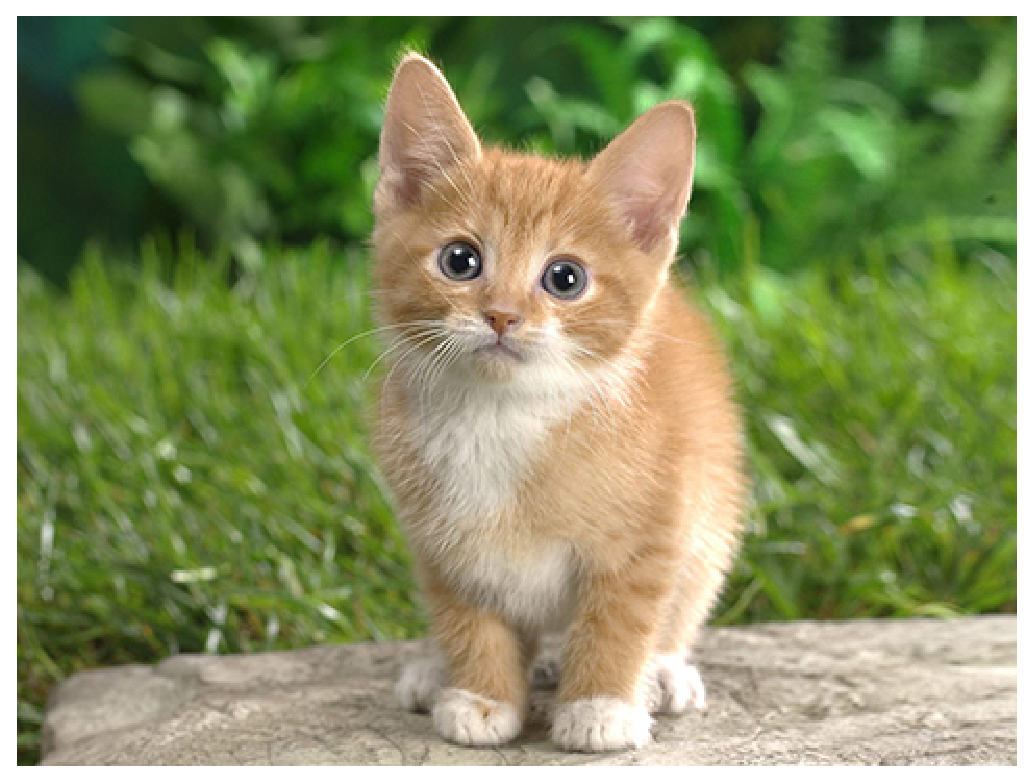
\includegraphics[width=50mm]{../02nd/fig/cat.eps}
   \caption{sample1}
	 \label{sample1}
\end{figure}
\begin{figure}[b]
\centering
    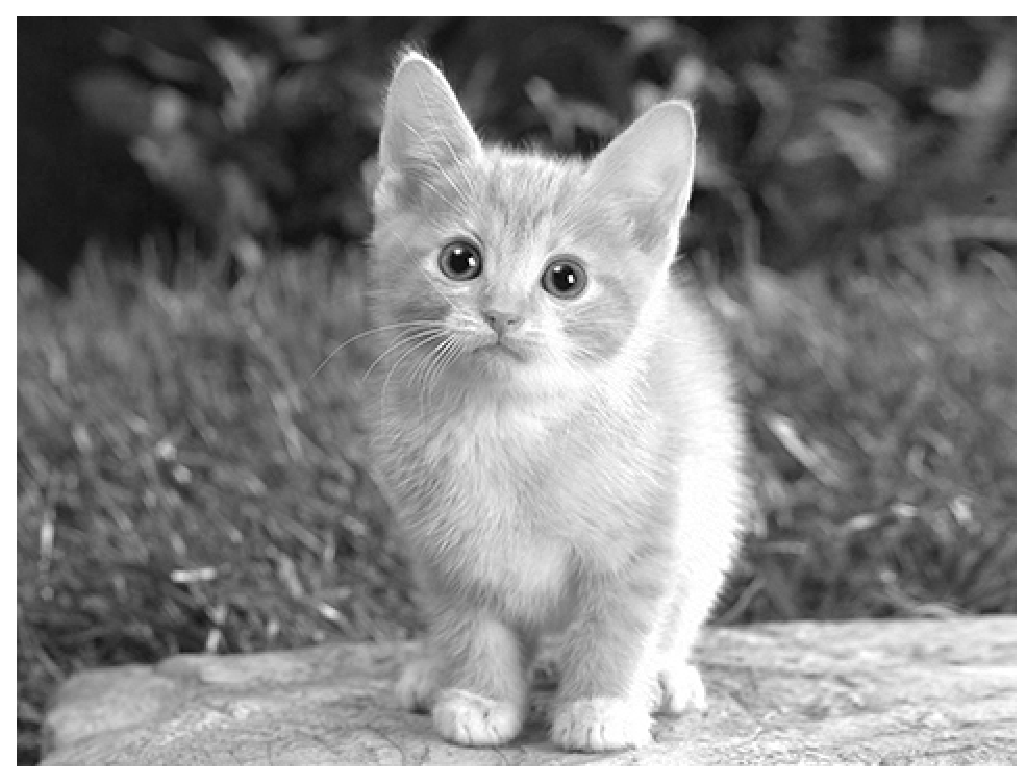
\includegraphics[width=50mm]{../02nd/fig/cat_gray.eps}
\caption{sample2}	 
 \label{sample2}
\end{figure}
\begin{figure}[b]
\centering
    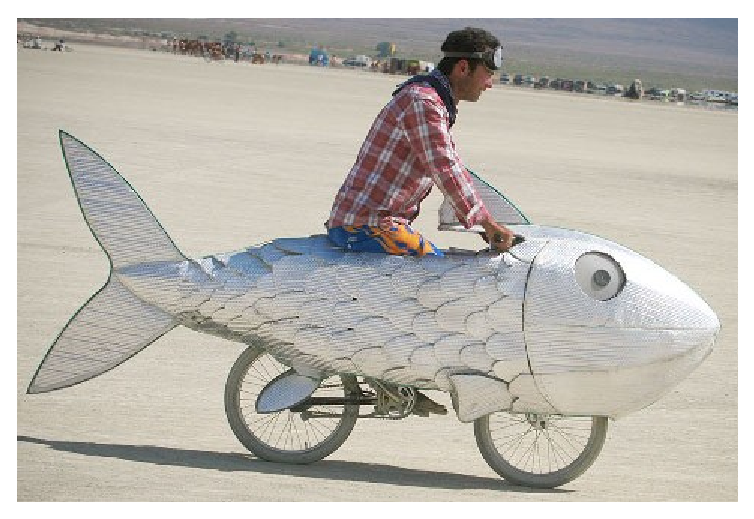
\includegraphics[width=50mm]{../02nd/fig/fish-bike.eps}
\caption{sample3}
\label{sample3}
\end{figure}

分類の実行
\begin{lstlisting}[basicstyle=\ttfamily\footnotesize, frame=single]
python show_result.py ../data/ilsvrc12/synset_words.txt result.npy
\end{lstlisting}

Fig.\ref{sample1}の実行結果
\begin{lstlisting}[basicstyle=\ttfamily\footnotesize, frame=single]
#1 | n02123045 tabby, tabby cat | 27.9%
#2 | n02123159 tiger cat | 21.9%
#3 | n02124075 Egyptian cat | 16.1%
\end{lstlisting}

Fig.\ref{sample2}の実行結果
\begin{lstlisting}[basicstyle=\ttfamily\footnotesize, frame=single]
#1 | n02342885 hamster | 54.7%
#2 | n02325366 wood rabbit, cottontail, cottontail rabbit | 17.2%
#3 | n02326432 hare | 16.4%
\end{lstlisting}

Fig.\ref{sample3}の実行結果
\begin{lstlisting}[basicstyle=\ttfamily\footnotesize, frame=single]
#1 | n04120489 running shoe |  6.9%
#2 | n04509417 unicycle, monocycle |  3.9%
#3 | n04482393 tricycle, trike, velocipede |  3.6%
\end{lstlisting}

\section{今後の課題}


\end{document}